% Example LaTeX document for GP111 - note % sign indicates a comment
\documentclass[12pt]{article}
% Default margins are too wide all the way around. I reset them here
\usepackage{amsmath}
%\usepackage{mathtools}
\usepackage{graphicx}
\usepackage[danish]{babel}
\usepackage{listings}
\usepackage{color}
\usepackage[utf8]{inputenc}
\usepackage{hyperref}
\usepackage{float}
%\usepackage[margin=1in]{geometry}

\definecolor{lightgray}{rgb}{.9,.9,.9}
\definecolor{darkgray}{rgb}{.4,.4,.4}
\definecolor{purple}{rgb}{0.65, 0.12, 0.82}

\lstdefinelanguage{JavaScript}{
	keywords={typeof, new, true, false, catch, function, return, null, catch, switch, var, if, in, while, do, else, case, break, eval, getElementById, exp, pow},
	keywordstyle=\color{blue}\bfseries,
	ndkeywords={class, export, boolean, throw, implements, import, this, document},
	ndkeywordstyle=\color{darkgray}\bfseries,
	identifierstyle=\color{black},
	sensitive=false,
	comment=[l]{//},
	morecomment=[s]{/*}{*/},
	commentstyle=\color{purple}\ttfamily,
	stringstyle=\color{red}\ttfamily,
	morestring=[b]',
	morestring=[b]"
}

\lstset{
	language=JavaScript,
	backgroundcolor=\color{lightgray},
	extendedchars=true,
	basicstyle=\footnotesize\ttfamily,
	showstringspaces=false,
	showspaces=false,
	numbers=left,
	numberstyle=\footnotesize,
	numbersep=9pt,
	tabsize=2,
	breaklines=true,
	showtabs=false,
	captionpos=t
}

\renewcommand\lstlistingname{Algoritme}
\addto{\captionsdanish}{\renewcommand{\abstractname}{Abstract}}
\numberwithin{equation}{section}
\addto{\captionsbahasa}{%
	\renewcommand*{\refname}{Daftar Pustaka}
}

\pagestyle{headings}

\begin{document}
\title{Numerisk Integration}
\author{Søren Fritzbøger 3F\\
HTX Hillerød - Erhversskolen Nordsjælland\\
Vejledt af Stig Nørskov Jacobsen og Christian Reinhold}
\renewcommand{\today}{2. Februar 2015}
\maketitle

\begin{abstract}
This article demonstrates a basic set of LaTeX formatting commands.
Compare the typeset output side-by-side with the input document.smøøre
\end{abstract}
\newpage
\tableofcontents
\newpage
\section{Indledning}
Når man skal bestemme arealet under en funktion, kan man finde det bestemte integral. Men for nogle funktioner er det ikke muligt at bestemme det bestemte integral. I dette tilfælde kan man bruge numerisk integration til tilnærmelsesvist at bestemme arealet under funktionen. I dette projekt vil jeg kort forklare hvad der menes med numerisk integration, og følgende redegøre for numerisk integration ved hjælp af Trapezmetoden og Simpsons metode. Efterfølgende vil jeg redegøre for, hvorledes metoderne kan omsættes til et IT-program og vurdere effektiviteten og nøjagtigheden af metoderne.
\\
Jeg vil redegøre for både Trapezmetoden og Simpsons metode, ved at udlede og bevise deres formler, og senere vise at de også kan beregne arealet under en funktion, der ikke direkte kan integreres. Jeg vil vurdere effektiviteten og nøjagtigheden af metoderne, ved først at omsætte dem til en algoritme, og herefter indsamle data vedrørende nøjagtighed og effektivitet. Jeg vil undersøge hvor lang beregningstiden er for hver funktion og sætte dem op mod hinanden. Jeg vil også undersøge nøjagtigheden for metoderne og tilhørende algoritme, ved at sammenligne med det bestemte integral.

\section{Forklaring af numerisk integration}
Numerisk integration kan også kaldes for tilnærmelsesvist bestemmelse af det bestemte integral $\int_{a}^{b}f(x)dx$.\footnote{\cite{numeriskintegration}} Normalt bruger man bestemte integraler til dette, men når funktionen er så avanceret, som f.eks. $f(x)=e^{-x^2}$, er det ikke muligt at bruge bestemt integration til at finde arealet.\footnote{\cite{2012matA}} Numerisk integration opdeler funktionen i mindre stykker, og udregner herefter arealet af stykkerne og finder summen. Der findes flere forskellige metoder til at udregne arealet. Blandt dem kan nævnes Midpunktsreglen, Trapezmetoden og Simpsons metode. Trapezmetoden og Simpsons metode, er de 2 der som regel er mest præcise, men det er selvfølgelig også de mest avancerede.

\section{Trapezmetoden}
\label{sec:trapezmetoden}
Trapezmetoden er en af flere metoder til at finde areal under en funktion. Det er en af de mere præcise metoder, da den, i modsætning til højre-, venstre- og middelsum, laver en trapez og ikke en firkant.
\subsection{Bevis for trapezmetoden}
Ved at bruge trapezmetoden kan vi tilnærmelsesvist finde det bestemte integral, selv for funktioner, hvor man ikke direkte kan bestemme det bestemte integral.\footnote{\cite[s. 13]{2012matA}} Et eksempel på dette er funktionen $f(x)=e^{-x^{2}}$.\footnote{\cite[s. 12]{2012matA}}
For at bestemme arealet under en funktion vil vi gerne nærme os det bestemte integral.
\begin{equation}
\int_{a}^{b}f(x)dx \nonumber
\end{equation}
Når $a<b$ og $f$ er kontinuerlig og differentiabel i intervallet $[a;b]$, kan vi bruge trapezmetoden til at udregne det tilnærmelsesvist bestemte integral, som er arealet under funktionen.\\
Som navnet trapezmetoden så fint hentyder til, opdeler vi vores funktion i en trapez, som vi udregner arealet af. Dette er illustreret på figur \ref{fig:trapezmetoden}
\begin{figure}[H]
\centering
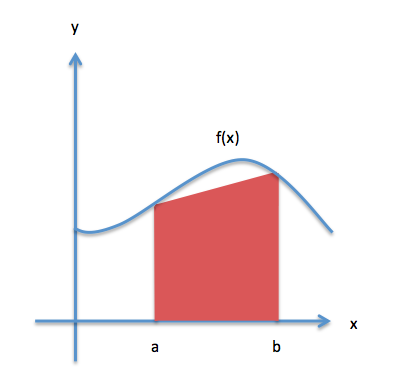
\includegraphics[scale=0.5]{Billeder/trapezmetoden.png}
\caption{Trapezmetoden}
\label{fig:trapezmetoden}
\end{figure}


På figur \ref{fig:trapezmetoden} kan man se, hvordan trapezmetoden opdeler en parabel i en trapez. Denne trapez har intervallet $[a;b]$. Længden $a=f(a)$ og længden $b=f(b)$. Formlen for arealet af en trapez ses i formel \eqref{eq:trapezareal}
\begin{equation}
\label{eq:trapezareal}
A=\frac{1}{2}h\cdot(a+b)
\end{equation}
\begin{figure}[H]
	\centering
	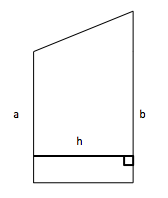
\includegraphics[scale=0.6]{Billeder/Trapez}
	\caption{Trapez}
	\label{fig:trapez}
\end{figure}

Som man kan se på figur \ref{fig:trapez}, er $a$ og $b$ er sidelænger og $h$ er højden. I et trapez er højden defineret som afstanden mellem de to parallelle linjestykker, i dette tilfælde $a$ og $b$, som man kan se illustreret på figur \ref{fig:trapez}
\\\\
Som man kan se på figur \ref{fig:trapez} svarer højden $h$ til afstanden mellem $a$ og $b$, som svarer til $h=b-a$. Når man indsætter henholdsvis $a$ og $b$ værdien ind i vores $f(x)$ funktion, får vi vores $y$ værdi, som svarer til længden af henholdsvis $a$ og $b$.
Hvis vi indsætter dette i arealet for en trapez, får vi derfor:
\begin{align}
A &= \frac{1}{2}h\cdot(a+b) &\Rightarrow \nonumber
\\ &= \frac{1}{2}(b-a) \cdot (a+b) &\Rightarrow \nonumber
\\ &= \frac{b-a}{2} (a+b) &\Rightarrow \nonumber
\intertext{i stedet for $a$ og $b$ indsættes højderne på trapezens sider, $f(a)$ og $f(b)$} \nonumber
\\ &= \frac{b-a}{2} (f(a)+f(b))
\\ \intertext{Arealet af denne trapez svarer tilnærmelsesvist til arealet under funktionen. Så derfor kan vi sige at arealet af trapezen tilnærmelsesvist svarer til værdien af det bestemte integral:} \nonumber
\\ \int_{a}^{b}f(x) &\approx \frac{b-a}{2} (f(a)+f(b))
\end{align}

\subsubsection{Opdeling i flere delintervaller}
\label{sec:opdelingtrapezmetoden}
Som man kan se på figur \ref{fig:trapezmetoden} er trapezmetoden meget upræcis i forhold til det bestemte integral. Dette kan man forbedre ved at dele intervallet $[a;b]$ op i flere delintervaller, $n$. Dvs. at vi deler vores funktion op i mindre intervaller, som vi så finder arealet af med trapezmetoden. Disse delintervaller kalder vi for $x_0, x_1, \cdots x_n$. Vi skal bruge højden på trapezen, som er længden af delintervallet $x_0 - x_1$. I dette tilfælde svarer det til:
\begin{align}
h = x_1-x_0 = x_2-x_1 = \cdots = x_n - x_{n-1}
\end{align}
Ud fra dette kan vi bestemme at højden, $h$, må svare til intervallet $[a;b]$ opdelt i $n$ intervaller:
\begin{align}
h=\frac{b-a}{n}
\end{align}
Det samlede areal under funktionen kan betegnes som summen af alle delintervallerne:
\begin{align}
A &= \lim\limits_{n \rightarrow \infty} \sum_{i=1}^{n} \frac{h}{2}(f(x_{i}) + f(x_{i+1}))
\approx \int_{a}^{b}f(x) &\text{hvor }h=\frac{b-a}{n}
\end{align}
Når n går mod uendelig bliver vores delinterval infinitesimalt lille, hvilket vil sige at summen af alle trapezarealerne nærmer sig det bestemte integral. Det bestemte integral svarer faktisk til at vi deler arealet op i uendelige små og uendelig mange led.
\\\\
For at udlede dette til formlen for trapezmetoden bliver vi nødt til at opskrive dette på en lidt anden måde.
\begin{align}
A &= \frac{h}{2}(f(x_0)+ f(x_1)) + \frac{h}{2}(f(x_1)+ f(x_2)) + \cdots + \frac{h}{2}(f(x_{n-1})+ f(x_n)) \nonumber
\\ &= h(\frac{1}{2}f(x_0) + \frac{1}{2}f(x_1)) + h(\frac{1}{2}f(x_1) + \frac{1}{2}f(x_2)) + \cdots + h(\frac{1}{2}f(x_{n-1}) + \frac{1}{2}f(x_n)) \nonumber
\\ &= h \cdot \frac{1}{2}f(x_0) + h \cdot \frac{1}{2}f(x_1) + h \cdot \frac{1}{2}f(x_1) + h \cdot \frac{1}{2}f(x_2) + \cdots + h \cdot \frac{1}{2}f(x_{n-1}) + h \cdot \frac{1}{2}f(x_n) \nonumber
\end{align}
Dette bliver reduceret til formlen for trapezmetoden\footnote{\cite[s. 14]{2012matA}} \eqref{eq:trapezmetoden}
\begin{align}
\label{eq:trapezmetoden}
\boxed{\int_{a}^{b}f(x) \approx \frac{h}{2}(f(x_0) + 2f(x_1) + \cdots + 2f(x_{n-1}) + f(x_n))} \\ \text{Hvor } h=\frac{b-a}{n} \nonumber
\end{align}

\section{Simpsons metode}
\label{sec:simpsonsmetode}
En anden metode til tilnærmelsesvist at udregne arealet under en funktion er simpsons-metoden, som virker ved at dele funktionen op i mindre parabler, man så finder arealet under. Denne metode er mere præcis end trapezmetoden\footnote{\cite[s. 15]{2012matA}}, og giver derfor et resultat som oftest har en meget lille afvigelse fra det korrekte resultat, det bestemte integral.
\subsection{Bevis for Simpsons metode}
Simpsons metode er som nævnt, en anden metode til tilnærmelsesvist at finde det bestemte integral, selv for funktioner, hvor man ikke direkte kan bestemme det bestemte integral. Med trapezmetoden, se afsnit \ref{sec:trapezmetoden}, brugte man en ret linje fra $f(a)$ til $f(b)$ i intervallet $[a;b]$, hvilket selvfølgelig ikke er helt præcis, da en funktion ikke nødvendigvis er ret. Med Simpsons metode opdeler man intervallet $[a;b]$ i en parabel ud fra 3 punkter, $a,b,c$.\footnote{\cite{simpsonsmetode}} Disse tre punkter kan bruges til at opstille en simplere parabel, som vi så kan regne arealet under. Parablens ligning ser således ud: $y=ax^2+bx+c$
\begin{figure}[H]
\centering
\includegraphics[width=0.6\linewidth]{Billeder/Simpsonsmetode}
\caption{Simpsons metode}
\label{fig:simpsonsmetode}
\end{figure}

Figur \ref{fig:simpsonsmetode} viser hvilke punkter vores parabel går gennem når vi har intervallet $[a;b]$. Ligesom med trapezmetoden kan man opdele funktionen i $n$ antal dele. Til at starte med går vi ud fra at $n=2$, for at gøre det nemt. \emph{I afsnit \ref{sec:simpsonopdeling} bliver der viderebygget på Simpsons metode med flere intervaller.}
Som man også kan se på figuren bliver $[a;b]$ delt op i to, hvor $\triangle x=h$. Dette viser sig også i punkterne som henholdsvis er $(-h,y_0)$, $(0,y_1)$ og $(h,y_2)$. Intervallet $[a;b]$ opdeles i $n$ antal delintervaller, som for dette tilfælde er 2, hvilket giver afstanden h mellem vores punkter.
\begin{align}
h &= \frac{b-a}{n} \nonumber
\\&= \frac{b-a}{2} &\text{Når } n=2
\end{align}
Vi ved at vores parabel går fra $-h$ til $h$ og at den har forskriften $y=ax^2+bx+c$. Dette simple udtryk for vores parabel kan vi bestemme det bestemte integral af, da vi ved at $f(x)=y$. Vi finder dermed det bestemte integral under en parabel med forskriften $y=ax^2+bx+c$ fra $-h$ til $h$\footnote{Der er brugt regneregler for integralregning til at finde det bestemte integral for funktionen, som kan ses i bilag 1}
\begin{align}
\label{eq:integral-hh}
A &=\int_{-h}^{h}f(x)dx \nonumber
\\ &=\left[ \frac{ax^3}{3} + \frac{bx^2}{2} + cx \right]_{-h}^{h} \nonumber
\\ &= \left( \frac{ah^3}{3} + \frac{bh^2}{2} + ch \right) - \left( -\frac{ah^3}{3} + \frac{bh^2}{2} - ch \right) \nonumber
\\ &= \frac{ah^3}{3} + \frac{ah^3}{3} + \frac{bh^2}{2} - \frac{bh^2}{2} + ch + ch \nonumber
\\ &= \frac{2ah^3}{3} + 2ch \nonumber
\\ &= \frac{h}{3}(2ah^2+6c)
\end{align}

Nu skal vi finde vores 2 ubekendte, som er $2ah^2$ og $c$. Dette kan vi gøre ved at opstille tre ligninger for parablen, $y=ax^2+bx+c$, med vores tre punkter $(-h,y_0)$, $(0,y_1)$, $(h,y_2)$ fra figur \ref{fig:simpsonsmetode}, hvor vi så har 3 ubekendte. Vi går ud fra at $y$ svarer til punkternes y-koordinat og $x$ til vores x-koordinat.

\begin{align}
\label{eq:ubekendte}
y_0 &= ah^2-bh+c & \text{Hvor } (x,y) &=(-h,y_0)
\\ y_1 &= a \cdot 0^2+b \cdot 0 +c \Rightarrow \nonumber
\\ y_1 &= c & \text{Hvor } (x,y) &=(0,y_1)
\\ y_2 &= ah^2+bh+c & \text{ } (x,y) &=(h,y_2)
\end{align}
Som man kan se på ligningen for $y_1$ \eqref{eq:ubekendte} har vi allerede fået isoleret vores $c$ værdi, som svarer til $c=y_1$
Vi vil gerne have isoleret $2ah^2$, og dette kan vi gøre ved at substituere $c$ ind i de to ligninger for $y_0$ og $y_2$ og derefter ligge dem sammen.
\\\\
Det gør vi således:
\begin{align}
y_0 &= ah^2 - bh + c &\Rightarrow &&\text{Hvor } c=y_1 \nonumber
\\ y_0 &= ah^2 -bh + y_1 & \Rightarrow \nonumber
\\ y_0-y_1 &= ah^2-bh
\label{eq:ah2-bh}
\\ \nonumber
\\y_2 &= ah^2 + bh + c &\Rightarrow &&\text{Hvor } c=y_1 \nonumber
\\y_2 &= ah^2 + bh + y_1 & \Rightarrow \nonumber
\\y_2 - y_1 &= ah^2 +bh
\label{eq:ah2+bh}
\end{align}
Ligning \eqref{eq:ah2-bh} og \eqref{eq:ah2+bh} ligges nu sammen, så vi kan isolere den sidste og manglende ubekendte, $2ah^2$.

\begin{align}
	y_2 - y_1 &= ah^2 - bh &+ \nonumber
\\	y_0 - y_1 &= ah^2 + bh \nonumber
\\ &&= \nonumber
\\ ah^2 -bh + bh &= y_2 + y_0 - y_1 - y_1 \Rightarrow \nonumber
\\ ah^2 &= y_2 + y_0 - 2y_1
\end{align}
$ah^2$ og $c$ substitueres nu ind i formel \eqref{eq:integral-hh} som ser således ud: $A = \frac{h}{3}(2ah^2+6c).$

\begin{align}
\label{eq:ensimpson}
A &= \frac{h}{3}(2ah^2+6c) \nonumber
\\&= \frac{h}{3}\left( \left( y_2+y_0-2y_1 \right) + 6 \cdot y_1 \right) \nonumber
\\&= \frac{h}{3}(y_0+4y_1+y_2)
\end{align}


%Ud fra ligning \eqref{integral-hh} kan vi lave vores parabel ved at opstille tre ligninger med 3 ubekendte, vha. vores 3 punkter: $(-h,y_0)$, $(0,y_1)$, $(h,y_2)$.
%De tre ligninger ser således ud:

\subsubsection{Opdeling i flere delintervaller}
Når vi deler vores interval op i flere delintervaller, dvs. at $n$ bliver større, kan vi finde summen af $n$ antal delintervaller mellem $[a;b]$.\footnote{\cite[s. 15-16]{2012matA}} Vi skal bruge 2 delintervaller for at finde vores parabel, og derfor skal $n$ være lige.\footnote{\cite[s. 15-16]{2012matA}} På figur \ref{fig:simpsonOpdeling} kan man se et eksempel på en opdeling med $n=4$, hvor vi faktisk har 2 parabler. En fra $y_0$ til $y_2$ gennem $y_1$ og en fra $y_2$ til $y_4$ gennem $y_3$.
\label{sec:simpsonopdeling}
\begin{figure}[H]
\centering
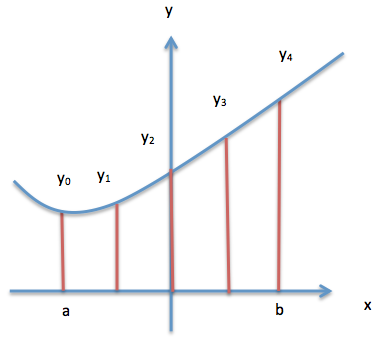
\includegraphics[width=0.6\linewidth]{Billeder/simpsonOpdeling}
\caption{Opdeling i flere delintervaller}
\label{fig:simpsonOpdeling}
\end{figure}

Ved hjælp af formel \eqref{eq:ensimpson} kan vi udregne arealet af en parabel fra $y_0$ til $y_2$. Men hvis vi udvider denne som man kan se på figur \ref{fig:simpsonOpdeling}, kan vi fortsætte simpsonsreglen fra $y_2$ til $y_4$, og dermed få det samlede areal for $[a;b]$ som går fra $y_0$ til $y_4$, som man kan se på figur \ref{fig:simpsonOpdeling}.
Summen af arealet fra $[a;b]$ når opdelingen $n=4$
\begin{align}
\label{eq:simpsonOpdeling}
A_{[a;b]} 	&= \frac{h}{3}(y_0 + 4y_1 + y_2) + \frac{h}{3}(y_2 + 4y_3 + y_4) \nonumber
\\ 			&= \frac{h}{3}(y_0 + 4y_1 + y_2 + y_2 +4y_3 +y_4) \nonumber
\\			&= \frac{h}{3}(y_0 + 4y_1 + 2y_2 + 4y_3 + y_4) & \text{Hvor } y=f(x)
\intertext{Det samme sker hvis vi har en opdeling på $n=6$}
A_{[a;b]}	&= \frac{h}{3}(y_0 + 4y_1 + 2y_2 + 4y_3 + 2y_4 + 4y_5 + y_6) & \text{Når } n=6
\label{eq:simpsonOpdeling6}
\end{align}
Ud fra dette kan vi opstille en ligning der siger at summen af alle delarealerne i intervallet $[a;b]$ opdelt i $n$ delintervaller tilnærmelsesvist må svare til det bestemte integral.
\begin{align}
A &= \lim\limits_{n \rightarrow \infty} \sum_{i=1}^{n/2} \frac{h}{3}(y_{i-2} + 4y_{i-1} + y_{i}) \approx \int_{a}^{b}f(x) &\text{hvor }h=\frac{b-a}{n}
\end{align}
Når n går mod uendelig bliver vores delinterval infinitesimalt lille, hvilket vil sige at summen af alle vores delintervaller, hvor vi har udregnet arealet under parablen. På den måde nærmer det, vha. Simpsons metode, udregnede areal tilnærmelsesvist det bestemte integral.
\\\\
For at udlede dette til formlen for Simpsons metode, skal vi kigge nærmere på formel \eqref{eq:ensimpson} og omskrive denne til at $n$ går mod uendelig.
\begin{align}
A	&= \frac{h}{3}(f(x)_0 + 4f(x)_1 + f(x)_2) \qquad \qquad \qquad \qquad \quad \text{Hvor } f(x)=y \text{ og når } n = 2 \nonumber
\\	&= \frac{h}{3}(f(x_0) + 4f(x_1) + f(x_2) + f(x_2) + 4f(x_3) + f(x_4)  	+ \cdots + f(x_{n-2}) + 4f(x_{n-1}) + f(x_n) ) \nonumber
\end{align}
Dette bliver reduceret til Simpsons metode\footnote{\cite[s. 16]{2012matA}} \eqref{eq:simpsonsmetode}
\begin{align}
\label{eq:simpsonsmetode}
\boxed{\int_{a}^{b} \approx \frac{h}{3}(f(x_0) + 4f(x_1) + 2f(x_2) + 4f(x_3) + \cdots + 2f(x_{n-2}) + 4f(x_{n-1}) + f(x_n) )}
\\ \text{Hvor } h=\frac{b-a}{h} \text{ og $n$ er lige} \nonumber
\end{align}

\pagebreak
\section{Numerisk integration og computere}
Når man skal omsætte en matematisk formel, til noget computeren kan forstå og regne med, skal man lave en såkaldt \emph{algoritme}. En algoritme er en forskrift til løsning af et matematisk eller logisk problem, hvor man kender antallet af beregningsskridt\footnote{\cite{version2:algoritme}[Version2.dk]}. I dette tilfælde er forskriften de 2 udledte formler \eqref{eq:trapezmetoden}, trapezmetoden, og \eqref{eq:simpsonsmetode}, Simpsons metode, fra afsnit \ref{sec:trapezmetoden} og \ref{sec:simpsonsmetode}, der tilnærmelsesvist bestemmer det bestemte integral. Samtidig kender vi også antallet af beregningsskridt, da dette er antallet af delintervaller $n$. Derfor kan vi med sikkerhed sige, at vi kan lave en algoritme der tilnærmelsesvist udregner arealet under en vilkårlig matematisk funktion.
Når man skal skrive en algoritme til en computer, skal dette gøres i et programmeringssprog\footnote{\cite{denstoredanske:algoritme}[Den store danske]}, som f.eks. JavaScript, PHP, C++, java osv. Hvert sprog kan bruges til forskellige ting og på forskellige enheder. Nogle programmeringssprog bruges til regulære computerprogrammer mens andre er udviklet til at fungere i en webbrowser som Chrome, Internet Explorer og lignende.
\\
Når man arbejder med algoritmer, er der nogle ting, som er meget vigtige at have styr på. Det ene er selvfølgelig at algoritmen giver et korrekt resultat, altså at den er nøjagtig, og det andet er hvor lang tid algoritmen bruger på udregningerne. Der skal være en fin balance mellem nøjagtigheden og effektiviteten. Nogle gange er det meget vigtigt at algoritmen er 100\% nøjatig, mens at andre algoritmer er så avancerede, at en 100\% nøjagtighed tager for lang tid. Nogle algoritmer kan være så komplekse og kræve så store beregningsmæssige ressourcer, at de ikke kan løses med de computere, vi har adgang til i dag.
\\\\
Jeg har brugt JavaScript til at opbygge mine algoritmer for Trapezmetoden og Simpsons metode. Fordelen ved JavaScript er at det kan køre i browseren, og det er derfor forholdsvist nemt for alle at køre. Samtidig er JavaScript et af de sprog, der har en mere simpel syntaks, så det er nemt at forstå, og det er derfor også meget tilgængeligt.

\subsection{Effektivitetsoptimering i JavaScript}
Når man skal skrive en algoritme, er det næsten umuligt ikke at have et såkaldt \emph{loop}. Et loop, løkke på dansk, er en kode, der kører så længe at en defineret erklæring passer. Den løkke jeg skal bruge til mine algoritmer, skal køre $n$ antal gange, altså den skal køre det antal gange, jeg har delt min funktion op i. I teorien kan n bevæge sig mod uendelig, men dette vil så også tage op mod uendelig tid. For at finde en 100\% præcis værdi af vores numeriske integration, kan vi godt risikere at vi kommer op på et delinterval på flere millioner. Derfor at det vigtigt at vi optimere løkken mest muligt, da det er en kode, der potentielt skal køre mange millioner gange. En måde at optimere løkken på er ved at vælge en while-løkke i stedet for en for-løkke. Et hurtigt eksperiment\footnote{\cite{forvswhile}} viser, at while-løkken i gennemsnit er en smule hurtigere\footnote{Det skal nævnes at det ikke er et 100\% korrekt eksperiment, da andre processer fra computeren, kan have haft en rolle i beregningstiden. Hvis man dog fjerner de meget afvigende resultater fra det samlede billede, er while-løkken stadig gennemsnitlig hurtigst.}. Samtidig udførte eksperimentet kun en meget simpel beregning, hvor den algoritme vi skal udregne, er meget mere avanceret. Derfor kan der være en stor besparelse i tid og beregningskraft, hvis man bruger en while-løkke i stedet for en for-løkke.


\subsection{Opbygning af algoritmerne}
Når man skal lave en algoritme til en matematisk funktion, er det vigtigt at have analyseret formlen først, så man kan skabe en præcis og effektiv algoritme. Jeg har udarbejdet en fungerende algoritme, som jeg har prøvet at effektivisere så meget som muligt. Derefter har jeg analyseret nøjagtigheden og effektiviteten af både metoden og algoritmen.
\subsubsection{Trapezmetoden}
Formlen for Trapezmetoden \eqref{eq:trapezmetoden}, som også kan ses på side \pageref{eq:trapezmetoden}, ser således ud:
\begin{align}
\int_{a}^{b}f(x) \approx \frac{h}{2}(f(x_0) + 2f(x_1) + \cdots + 2f(x_{n-1}) + f(x_n)) &&\text{Hvor } h=\frac{b-a}{n} \nonumber
\end{align}
Når man analyserer Trapezmetoden i forhold til at skulle lave en algoritme, er der et par ting man skal have fokus på. For det første er $\frac{h}{2}$ uden for parentesen hvilket gør, at vi til sidst i algoritmen kan udregne summen af delarealerne ganget med $\frac{h}{2}$. En anden ting er, at første og sidste punkt, henholdsvis $x_0$ og $x_n$ ikke skal ganges med 2 ligesom resten af delarealerne. Derfor kan vi sætte disse to uden for vores hoved-løkke, hvilket gør at vi ikke skal bekymre os om dem i løkken.
Ud fra denne korte analyse har jeg skrevet min algoritme for Trapezmetoden i intervallet $[a;b]$ og med antallet af delintervaller $n$.
\begin{lstlisting}[caption="udregnArealTrapezmetoden()"]
function udregnArealTrapezmetoden(a,b,n) {
	var h = (b-a)/n;
	var funktion = document.getElementById("funktion").value;
	
	var w = 1;
	var x = a;
	
	var areal = eval(funktion);
	while(w < n) {
		x = x + h;
		areal += 2*eval(funktion);
		w++;
	}
		
	x = b;
	areal += eval(funktion);
	areal = (h/2)*areal;
		
	return areal;
}
\end{lstlisting}

Min algoritme er opbygget som en funktion med variabler $a,b,n$. $a$ er startintervallet, $b$ er slutintervallet og $n$ er antal delintervaller, præcis som i formlen for Trapezmetoden. $h$ defineres præcis som i Trapezmetoden, dvs $h=\frac{b-a}{n}$. Variablen $funktion$ tager værdien fra et input der har id'et "funktion", som indeholder vores funktion formateret som JavaScript. Et eksempel på dette ses her for $f(x) = e^{-x^2}$
\begin{lstlisting}
Math.exp(Math.pow(-x,2))
\end{lstlisting}
Variablen $w$ er vores tæller som starter på 1. $x$ bliver sat til a, da vi skal substituere $x$ ind i vores funktion. På linje 8 udregnes arealet af $x_1$, som sker før vores løkke, som nævnt i analysen. På linje 9 starter vores løkke, som kører så længe w er mindre end n. Dvs. at løkken kører lige ind til vi når sidste punkt, $x_{n-1}$, så vi kan regne $x_n$ særskilt. Inde i løkken bliver x sat til længden af delintervallet, $h$ lagt sammen med sig selv, når vi finder den næste x-værdi i intervallet. Så udregnet arealet af delintervallet og ligges til variablen $areal$. Derefter lægger vi 1 til w, så den tæller op mod n.
Efter løkken har kørt, sætter vi $x$ til at være vores sidste værdi, $b$, og regner arealet for det sidste delinterval. Til sidst ganges hele det udregnede delareal med $\frac{h}{2}$ for at finde det samlede areal. Funktionen returnerer arealet til sidst.


\subsubsection{Simpsons metode}
Formlen for Simpsons metode \eqref{eq:simpsonsmetode}, som også kan ses på side \pageref{eq:simpsonsmetode}, ser således ud:
\begin{align}
\int_{a}^{b} \approx \frac{h}{3}(f(x_0) + 4f(x_1) + 2f(x_2) + 4f(x_3) + \cdots + 2f(x_{n-2}) + 4f(x_{n-1}) + f(x_n) ) \nonumber
\\ \text{Hvor } h=\frac{b-a}{h} \text{ og $n$ er lige} \nonumber
\end{align}
Simpsons metode ser en del anderledes ud end Trapezmetoden, så derfor skal den analyseres anderledes, og algoritmen kommer formentlig også til at blive mere avanceret.\\
Igen har vi h uden for parentesen, dog bare $\frac{h}{3}$ i stedet. Samtidig skal punkt $x_0$ og $x_n$ ikke ganges med noget, så de kan også beregnes uden for løkken. En ting der skal lægges meget mærke til ved Simpsons metode, er at den skifter mellem at multiplicere med 4 og 2. En måde at beskrive det er, at alle ulige skal ganges med 4 og lige med 2. Derfor skal løkken indeholde en \emph{if/else} sætning, der tjekker om det er et lige eller ulige antal vi beregner på. Ud fra denne analyse, har jeg skrevet min algoritme for Simpsons metode i intervallet $[a;b]$ og med antallet af delintervaller $n$

\begin{lstlisting}[caption="udregnArealSimpsonsMetode()"]
function udregnArealSimpsonsMetode(a,b,n) {
var h = (b-a)/n;
var funktion = document.getElementById("funktion").value;

var w = 1;
var x = a;

var areal = eval(funktion);
while(w < n) {
	x = x +h;
	if(w%2 == 0)
		areal += 2*eval(funktion);
	else
		areal += 4*eval(funktion);
	
	w++;
}

x = b;
areal += eval(funktion);
areal = (h/3)*areal;

return areal;
}
\end{lstlisting}

Igen er algoritmen opbygget som en funktion med intervallet $[a;b]$ og antal delintervaller $n$. De første 8 linjer er præcis det samme som i Algoritme 1: "udregnArealSimpsonsMetode()", hvor der defineres forskellige variabler, og arealet for $x_1$ udregnes. Det næste er while-løkken på linje 9 som kører så længe w er mindre end antal delintervaller $n$. Først sættes x til at være næste delinterval, og dernæst tjekkes der om tælleren, $w$, er et lige eller ulige tal. Dette gør den vha. modulus funktionen, (\emph{skrives \% i JavaScript}), som er en matematisk funktion. Modulus svarer til det positive heltal, der er i rest, når man dividerer. Så når man tager modulus 2 af et tal, giver det enten en rest på 1, når tallet af ulige, og ellers en rest på 0, da alle lige tal går op i 2. Arealet af delintervallet regnes så ud fra denne \emph{if/else}-sætning, hvor lige ganges med 2 og ulige med 4.
\\Resten af koden afviger kun fra algoritmen til Trapezmetoden ved at gange det samlede udregnede areal med $\frac{h}{3}$ som det står i Simpsons metode \eqref{eq:simpsonsmetode}.
\subsection{Vurdering af effektiviteten og nøjagtigheden}
Helt grundlæggende vil jeg 
Når jeg skal vurdere nøjagtigheden, vil jeg både vurdere selve metoden og algoritmen. Hvis algoritmen er skrevet korrekt, burde der ikke være forskel på nøjagtigheden i forhold til metoden. Jeg vil undersøge nøjagtigheden ud fra resultatet af algoritmen/metoden opdelt i forskellige delintervaller, $n$, i forhold til det bestemte integral.
\\Effektiviteten kan være svær at vurdere, da jeg ikke har noget at stille mine data op imod. Jeg har undersøgt hvor lang tid det tager, at køre algoritmen med forskellige delintervaller. Denne tid kan sammenlignes med nøjagtigheden af algoritmen, og ud fra det vil jeg vise en sammenhæng mellem præcision og hastighed.\\
Jeg har udvalgt 2 funktioner som minder om hinanden, dog er den ene en del mere avanceret end den anden. Den ene er $e^x$ og den anden $e^{-x^2}$. Den anden funktion, $e^{x^2}$, er en af de funktioner man ikke kan bestemme det bestemte integral af, mens den første er simpel at bestemme. Til at bestemme arealet der er så tæt på det bestemte integral som muligt for $e^{-x^2}$, har jeg brugt Mathcad\footnote{Mathcad bruger også Numerisk integration til at udregne arealet, men delintervallet i Mathcad er meget højt, og derfor går jeg ud fra at tallet er præcist nok til at sammenligne med.}, som har givet den værdi der står i tabel \ref{tab:trapezmetodenex2} og \ref{tab:simpsonsmetodeex2}
\subsubsection{Nøjagtighed og effektivitet når $f(x)=e^x$}
Funktionen $e^x$ er en forholdsvis simpel funktion, som er nem at bestemme integralet af. Hvis vi sammenligner resultater fra Trapezmetoden og Simpsons metode fra tabel \ref{tab:trapezmetodenex} og \ref{tab:simpsonsmetodeex}. Hvis vi kigger på nøjagtigheden af metoderne og algoritmerne, tegner der sig et klart billede. Simpsons metode er den mest præcise, og rammer allerede det bestemte integral ved $n=14$ som man kan se på tabel \ref{tab:simpsonsmetodeex}. Derimod skal Trapezmetoden bruge et antal delintervaller på hele 180, for at bestemme det korrekte areal.
\begin{table}[H]
	\caption {Nøjagtighed af Trapezmetoden for $f(x)=e^x$ i intervallet $[-1;3]$}
	\label{tab:trapezmetodenex}
\begin{center}
\begin{tabular}{|c|r@{.}l|r @{.} l|r @{.} l|}
	\hline $n$ & \multicolumn{2}{|c|}{Beregningstid} & \multicolumn{2}{|c|}{Trapezmetoden} & \multicolumn{2}{|c|}{Bestemt integral}
	\\
	\hline 2 & 0&05ms & 25&89 & 19&718\\ 
	\hline 4 & 0&016ms & 21&334 & 19&718\\ 
	\hline 10 & 0&019ms & 19&98 & 19&718\\ 
	\hline 20 & 0&022ms & 19&738 & 19&718\\ 
	\hline 40 & 0&029ms & 19&734 & 19&718\\ 
	\hline 180 & 0&088ms & 19&718 & 19&718\\ 
	\hline 
\end{tabular}
\end{center}
\end{table}
\begin{table}[H]
	\caption {Nøjagtighed af Simpsons metode for $f(x)=e^x$ i intervallet $[-1;3]$} 
	\label{tab:simpsonsmetodeex}
	\begin{center}
		\begin{tabular}{|c|r@{.}l|r @{.} l|r @{.} l|}
			\hline $n$ & \multicolumn{2}{|c|}{Beregningstid} & \multicolumn{2}{|c|}{Simpsons metode} & \multicolumn{2}{|c|}{Bestemt integral}
			\\ 
			\hline 2 & 0&0179ms & 20&884 & 19&718\\ 
			\hline 4 & 0&026ms & 19&815 & 19&718\\ 
			\hline 10 & 0&040ms & 19&72 & 19&718\\ 
			\hline 14 & 0&050ms & 19&718 & 19&718\\ 
			\hline 
		\end{tabular}
	\end{center}
\end{table}
Hvis man kigger på effektiviteten af algoritmerne, altså hvor stor beregningstid de har, kan man se at trapezmetoden er hurtigere per delinterval. Dog skal den bruge 0.088ms for at finde det korrekte areal, mod 0.050ms for Simpsons metode.
\\
Ud fra disse observationer og resultaterne fra tabel \ref{tab:trapezmetodenex} og \ref{tab:simpsonsmetodeex} kan vi sige, at Trapezmetoden har den korteste beregningstid per delinterval, men at Simpsons metoden er mest effektiv, og giver det mest nøjagtige resultat når $f(x)=e^x$.

\subsubsection{Nøjagtighed og effektivitet når $f(x)=e^{-x^2}$}
$f(x)=e^{-x^2}$ er en del mere avanceret funktion end $e^x$. Dette kan man også se på tabel \ref{tab:trapezmetodenex2} og \ref{tab:simpsonsmetodeex2}, da Simpsons metoden først finder det rigtige resultat ved $n=252$. Dog har trapezmetoden problemer ved at finde det korrekte areal, da den selv ved 2000 delintervaller, stadig ikke har fundet det Mathcad-udregnede areal.
\begin{table}[H]
	\caption {Nøjagtighed af Trapezmetoden for $f(x)=e^{-x^2}$ i intervallet $[-1;3]$} 
	\label{tab:trapezmetodenex2}
	\begin{center}
		\begin{tabular}{|c|r@{.}l|r @{.} l|l|}
			\hline $n$ & \multicolumn{2}{|c|}{Beregningstid} & \multicolumn{2}{|c|}{Trapezmetoden} & Bestemt integral
			\\
			\hline 2 & 0&020ms & 8111&239 & 1446.008\\ 
			\hline 4 & 0&020ms & 4111&218 & 1446.008\\ 
			\hline 10 & 0&021ms & 2032&925 & 1446.008\\ 
			\hline 20 & 0&022ms & 1603&752 & 1446.008\\ 
			\hline 40 & 0&036ms & 1486&247 & 1446.008\\ 
			\hline 180 & 0&090ms & 1448&008 & 1446.008\\
			\hline 400 & 0&182ms & 1446&413 & 1446.008\\
			\hline 2000 & 1&008ms & 1446&024 & 1446.008\\
			\hline
		\end{tabular}
	\end{center}
\end{table}

\begin{table}[H]
	\caption {Nøjagtighed af Simpsons metode for $f(x)=e^{-x^2}$ i intervallet $[-1;3]$} 
	\label{tab:simpsonsmetodeex2}
	\begin{center}
		\begin{tabular}{|c|r@{.}l|r @{.} l|l|}
			\hline $n$ & \multicolumn{2}{|c|}{Beregningstid} & \multicolumn{2}{|c|}{Simpsons metode} & Bestemt integral
			\\ 
			\hline 2 & 0&018ms & 5411&117 & 1446.008\\ 
			\hline 4 & 0&020ms & 2777&877 & 1446.008\\ 
			\hline 10 & 0&039ms & 1593&515 & 1446.008\\ 
			\hline 20 & 0&025ms & 1460&694 & 1446.008\\ 
			\hline 40 & 0&037ms & 1447&079 & 1446.008\\ 
			\hline 180 & 0&098ms & 1446&011 & 1446.008\\
			\hline 252 & 0&129ms & 1446&008 & 1446.008\\
			\hline 
		\end{tabular}
	\end{center}
\end{table}
Igen er trapezmetoden den hurtigste per delinterval, men det bliver overskygget af Simpsons metode til at udregne det nøjagtige resultat hurtigst og ved færrest delintervaller.
\\\\
Alt i alt kan man med sikkerhed sige, at Simpsons metode både er den mest nøjagtige og effektive metode. Den er både hurtigst til at finde det rigtige resultat, og finder også det rigtige resultat ved færre delintervaller.

\section{Konklusion}
I denne opgave har jeg kort forklaret om numerisk integration og redegjort for de to numeriske metoder Trapezmetoden og Simpsons metode. Derudover har jeg omsat metoderne til en computer algoritme, hvor jeg har vurderet effektiviteten og nøjagtigheden af både metoden og algoritmen.

\clearpage
%\addcontentsline{toc}{section}{Litteratur}
\section{Litteraturliste}
\begin{thebibliography}{9}
\bibitem{numeriskintegration}
	Den Store Danske - Mogens Esrom Larsen,
	\emph{Numerisk Integration}
	\url{http://www.denstoredanske.dk/It,_teknik_og_naturvidenskab/Matematik_og_statistik/It_og_numerisk_analyse/numerisk_integration}
	

\bibitem{simpsonsmetode}
	Interactive Maths - Murray Bourne,
	\emph{Simpson's Rule}
	\url{http://www.intmath.com/integration/6-simpsons-rule.php}
	
\bibitem{2012matA}
	Undervisningsministeriet,
	\emph{Forberedelse til Matematik A højere teknisk eksamen 2012}
	\url{http://uvm.dk/~/media/UVM/Filer/Udd/Gym/PDF12/Proever\%20og\%20eksamen/120608\%20Mat\%20A\%20htx\%20Forberedelsesmateriale.pdf}
	
\bibitem{version2:algoritme}
	Version2.dk - Klaus Hansen og Casper Thomsen,
	\emph{Leksikon: Algoritme}
	\url{http://www.version2.dk/leksikon/Algoritme}
	
\bibitem{denstoredanske:algoritme}
	Den Store Danske - Jens Clausen og senere af Uffe Rasmussen,
	\emph{Algoritme}
	\url{http://www.denstoredanske.dk/It,_teknik_og_naturvidenskab/Informatik/Software,_programmering,_internet_og_webkommunikation/algoritme}
\bibitem{forvswhile}

	Stoimen's web log,
	\emph{JavaScript Performance: for vs. while}
	\url{http://www.stoimen.com/blog/2012/01/24/javascript-performance-for-vs-while/}
\end{thebibliography}

\section{Kildekritik}
Når man skriver faglige projekter som dette, baseret på fakta, er man nødt til at have pålidelige og korrekte kilder. Derfor er kildekritik en essentiel del af det at skrive skriftlige opgaver. 
De kilder jeg har anvendt, har hovedsageligt være leksika-internetsider, hvor kilderne er så troværdige som muligt. Her snakker jeg om Den store danske, som bliver udgivet af Gyldendals. Den store danske er, modsat f.eks. Wikipedia, en leksikon side hvor brugerne ikke selv kan rette i indholdet, og dermed bliver vedligeholdt af udvalgt personale fra Gyldendals, hvilke sikrer korrekte data. 
Jeg har også benyttet mig af et professoroplæg, omhandlende det skrå kast, som er bygget op således at det kan anvendes som baggrund til et studieprojekt. Kilden har derfor været meget relevant for mit projekt, og har samtidigt en høj troværdighed, grundet forfatterens profession. Dog har jeg dobbelttjekket de vigtigste data, for at være helt sikker, og jeg har derfor stor tiltro til kilden. 
Kilderne fra Nasa er også meget troværdige kilder, da internet siderne for det første er skrevet af Nasa og for det andet ligger på et specielt domæne (.gov), der er reserveret til regeringen i USA. Dette betyder at både Nasa og USA ligger navn til kilden, hvilket gør den sikker.  
På trods af at det har været svært at finde relevante bøger, har jeg så vidt muligt forsøgt at holde til bøger som første informationskilde. Dette er da bøger generelt har en højere troværdighed en hjemmesider, da de kræver mere at producere, og ikke bare kan ændres efter publikation. Ved oven i at vælge bøger som bruges i undervisningen, er bøgerne også blevet godkendt af undervisningsministeriet, hvilket må betyde at deres indhold er yderst kvalificeret.
\section{Bilag}
\subsection{Bilag 1 - Regneregler for integralregning}
\begin{center}
	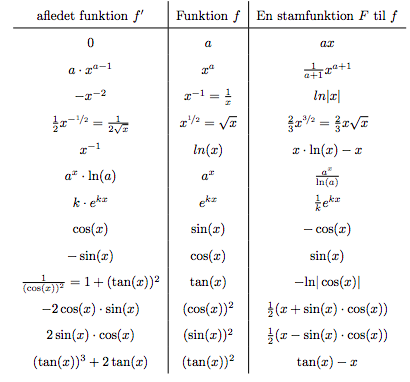
\includegraphics[width=0.9\linewidth]{Billeder/Integralregneregler}
\end{center}



\end{document}